\documentclass[conference]{IEEEtran}

\IEEEoverridecommandlockouts
\usepackage{cite}
\usepackage{amsmath,amssymb,amsfonts}
\usepackage{algorithmic}
\usepackage{graphicx}
\usepackage{textcomp}
\usepackage{xcolor}
\usepackage{booktabs}
\usepackage{url}
\usepackage{multirow}
\usepackage{microtype}
\usepackage{balance}

\def\BibTeX{{\rm B\kern-.05em{\sc i\kern-.025em b}\kern-.08em
    T\kern-.1667em\lower.7ex\hbox{E}\kern-.125emX}}

\begin{document}

\title{Multi-Stream Recommendation at Extreme Catalog Scale with Per-User Score Normalization}

\author{
    \IEEEauthorblockN{
        Aastha\IEEEauthorrefmark{1},
        Dhruv Gandhi\IEEEauthorrefmark{2},
        Rohit\IEEEauthorrefmark{3},
        Hrishikesh\IEEEauthorrefmark{4}, and
        Madhav\IEEEauthorrefmark{5}
    }
    \IEEEauthorblockA{
        Department of Computer Engineering\\
        Mukesh Patel School of Technology Management and Engineering (MPSTME)\\
        Mumbai, India\\
        Email: \{\IEEEauthorrefmark{1}aastha, \IEEEauthorrefmark{2}dhruv,
        \IEEEauthorrefmark{3}rohit, \IEEEauthorrefmark{4}hrishikesh,
        \IEEEauthorrefmark{5}madhav\}@nmims.in
    }
}

\maketitle

\begin{abstract}
Large-scale implicit-feedback music recommendation systems operate under conditions of extreme catalog scale, severe interaction sparsity, and heterogeneous signals spanning latent collaborative patterns, social tag semantics, and temporal recency dynamics. When merging heterogeneous retrieval streams across a catalog exceeding one million items, differences in score dispersion and dynamic range across users frequently lead to suboptimal ranking fusions. In this paper, we investigate a Global Normalized Multi-Stream Arbiter architecture evaluated on the Last.fm 1K listening dataset containing $19,150,865$ interaction events and $1,505,185$ unique observed tracks, evaluated over a filtered candidate catalog of $1,493,688$ tracks. The system integrates artist-level social tag semantics from HetRec 2011 ($2,299$ vocabulary tags covering $594,225$ catalog items). The architecture combines three distinct predictive signals: (1) an implicit MSVD/ALS collaborative model with log-confidence scaling, (2) an artist-level TF-IDF tag semantic affinity stream, and (3) a time-decayed temporal recency preference stream. To address score scale incompatibility across users without allocating dense user-item matrices, we introduce per-user min-max normalization on the collaborative stream prior to global weighted multi-stream fusion. Evaluation is conducted under a strict, chronologically ordered, zero-leakage split across $518$ evaluable test users over the full $1.49\text{M}$-track candidate catalog. On the complete test set, the Global Normalized Arbiter achieves an NDCG@10 of $0.007414$, representing a $+16.384\%$ descriptive improvement over Base MSVD ($0.006370$), a $+244.648\%$ relative improvement over the Popularity baseline ($0.002151$, Wilcoxon $p = 0.0447$, Cohen's $d = 0.1084$), and a $+24.480\%$ descriptive improvement over unnormalized fixed fusion ($0.005932$, $p = 0.1181$). Cohort analysis indicates that the multi-stream signals provide a $+50.472\%$ descriptive NDCG@10 gain ($0.017421$ vs.\ $0.011578$) for low-activity users ($2$--$2,090$ training plays). Exact sparse top-$K$ retrieval executes in $96.48\text{ ms}$ per user query ($10.36\text{ queries/sec}$ per CPU core) with verified sparse memory safety.
\end{abstract}

\begin{IEEEkeywords}
Recommender systems, implicit feedback, matrix factorization, alternating least squares, multi-stream fusion, score normalization, temporal preference decay, Last.fm, HetRec.
\end{IEEEkeywords}

\section{Introduction}
\IEEEPARstart{I}{mplicit-feedback} recommendation systems in music streaming platforms operate in an environment characterized by very large catalog sizes, non-negative observational feedback, and pronounced temporal and semantic variability~\cite{hu2008collaborative,celma2008music}. In platforms such as Last.fm, users interact with catalogs containing millions of tracks, but individual consumption profiles cover only a small fraction of available items, resulting in interaction matrix sparsity exceeding $99.99\%$.

Modern recommender systems frequently leverage latent factor models, such as Matrix Factorization solved via Alternating Least Squares (ALS) with implicit confidence transformations~\cite{hu2008collaborative,koren2009matrix}. While collaborative filtering effectively identifies global behavioral co-occurrences, it faces practical challenges when deployed in isolation at extreme scale:
\begin{enumerate}
    \item \textbf{User Interaction Sparsity:} Users with limited interaction histories lack sufficient collaborative density for accurate latent factor estimation.
    \item \textbf{Temporal Non-Stationarity:} User consumption exhibits recency dynamics, short-term listening bursts, and preference drift over time~\cite{koren2010collaborative}.
    \item \textbf{Score-Scale Incompatibility in Hybrid Systems:} Combining latent collaborative dot-products with external knowledge sources (e.g., social tag profiles) and temporal affinity vectors is impaired by divergent score distributions and non-standardized dynamic ranges across different users.
\end{enumerate}

To investigate whether these heterogeneous signals can be combined effectively under an extreme-catalog setting, we evaluate a \textbf{Global Normalized Multi-Stream Arbiter} recommendation framework designed for large-scale, full-catalog ranking. Our approach formulates top-$K$ track recommendation as the arbitration of three complementary streams:
\begin{itemize}
    \item \textbf{Collaborative Factorization Stream:} An implicit MSVD/ALS collaborative model mapping users and tracks into a 64-dimensional latent space via confidence-weighted ALS.
    \item \textbf{Stream A (Artist-Tag Semantic Affinity):} A content-based retrieval stream matching user listening history to artist-level social tags from the HetRec 2011 Last.fm dataset~\cite{cantador2011hetrec} using TF-IDF weighting and cosine projections.
    \item \textbf{Stream B (Temporal Recency Preference Modeling):} An exponentially decayed interaction affinity stream that captures immediate recency bias relative to pre-evaluation reference timestamps.
\end{itemize}

A key operational component of this work is \textbf{per-user score normalization}. Linear fusion of unnormalized collaborative scores and auxiliary scores can cause score dominance or ranking distortion due to variance in latent dot-product magnitudes across dense versus sparse users. We evaluate per-user min-max normalization on the collaborative stream prior to global fusion to align score dynamic ranges.

We evaluate the system under a \textbf{strict chronological zero-leakage protocol} over the entire $1,493,688$-item candidate catalog using $19,150,865$ listening events from the Last.fm 1K dataset~\cite{celma2008music}. Unlike sampled evaluations that evaluate against small subsets of negative items~\cite{cremonesi2010performance}, our evaluation ranks all $1.49\text{M}$ candidates for each evaluable test user. Furthermore, we report a statistical evaluation utilizing non-parametric Wilcoxon signed-rank tests~\cite{wilcoxon1945individual} and 10,000-sample bootstrap confidence intervals~\cite{efron1994introduction}, establishing empirical boundaries for all observed performance comparisons.

\section{Related Work}
\subsection{Implicit Feedback Collaborative Filtering}
Implicit feedback (e.g., listening counts, clicks, dwell time) differs from explicit ratings because non-interactions represent an unobserved mixture of negative preference and lack of exposure~\cite{steck2010training,liang2016modeling}. The formulation of Hu, Koren, and Volinsky (HKV)~\cite{hu2008collaborative} addressed implicit matrix factorization by introducing binary preference variables $p_{ui} \in \{0, 1\}$ coupled with confidence weights $c_{ui} = 1 + \alpha r_{ui}$. The resulting least-squares objective with L2 regularization is solved via Alternating Least Squares (ALS) with an $\mathcal{O}(f^2 |R| + f^3 |I|)$ per-iteration complexity, where $f$ is latent dimensionality. Extensions such as Bayesian Personalized Ranking (BPR)~\cite{rendle2012bpr} optimize pairwise ranking criteria directly. In this work, we employ an implicit MSVD/ALS collaborative model utilizing logarithmic confidence scaling $c_{ui} = 1 + \kappa \ln(1 + r_{ui})$ to stabilize confidence estimation across heavy-tailed listening play counts.

\subsection{Tag-Aware and Content-Augmented Recommendation}
Social tagging systems allow users to annotate artists, albums, and tracks with descriptive keywords. The HetRec 2011 benchmark~\cite{cantador2011hetrec} established standardized artist-level social tag assignments from Last.fm, enabling vector-space modeling of artist genres, eras, and stylistic descriptions. Prior literature has explored tensor factorization~\cite{rendle2012bpr} and hybrid linear models to incorporate tag information into collaborative filtering. However, when scaling to millions of candidate items, many tracks lack rich track-level annotations. Propagating artist-level tags across candidate tracks via TF-IDF representations provides an auxiliary semantic channel, while requiring handling of tag sparsity and vocabulary dispersion.

\subsection{Temporal Dynamics in Recommender Systems}
User preferences in music streaming exhibit multi-scale temporal non-stationarity, ranging from short-term repetition to long-term drift~\cite{koren2010collaborative}. Koren~\cite{koren2010collaborative} introduced TimeSVD++, parameterizing user and item biases as continuous functions of time. In fast-paced listening domains, exponential recency decay applied directly to interaction play counts provides a non-parametric mechanism to prioritize recent musical affinity without requiring complex non-linear parameter estimation.

\subsection{Multi-Stream Fusion and Score Calibration}
Hybrid recommendation architectures combine heterogeneous retrieval models (collaborative, content, popularity, session)~\cite{sarwar2001item}. A known challenge in hybrid fusion is score calibration. Unnormalized collaborative dot-products $x_u^T y_i \in (-\infty, \infty)$ vary across users depending on vector norms and interaction density. In contrast, cosine-based tag similarity scores are bounded in $[0, 1]$, and temporal affinity scores scale with decay functions. Without per-user normalization, global linear blending parameters $\sum w_m = 1$ can lead to inconsistent trade-offs across distinct user activity cohorts.

\section{Problem Formulation}
Let $\mathcal{U} = \{u_1, u_2, \dots, u_{|\mathcal{U}|}\}$ denote the set of users and $\mathcal{I} = \{i_1, i_2, \dots, i_{|\mathcal{I}|}\}$ denote the full candidate item catalog. The system observes an implicit event log $\mathcal{D} = \{(u, i, t, r_{ui})\}$, where each record represents user $u$ playing track $i$ at timestamp $t$ with aggregate count $r_{ui} \in \mathbb{N}_{\ge 1}$.

For a target user $u \in \mathcal{U}$ evaluated at test time, let $\mathcal{H}_u \subset \mathcal{I}$ denote the set of items consumed by user $u$ during training and validation periods. The objective is to produce an ordered recommendation list of top-$K$ candidate tracks $\text{Top-}K(u)$ from the unconsumed candidates $\mathcal{I} \setminus \mathcal{H}_u$:
\begin{equation}
\text{Top-}K(u) = \operatorname{arg\,topK}_{i \in \mathcal{I} \setminus \mathcal{H}_u} \hat{r}_{ui},
\end{equation}
where $\operatorname{arg\,topK}$ selects the $K$ items with the highest predicted scores $\hat{r}_{ui}$, sorted in descending order of score, and $\hat{r}_{ui}$ is the multi-stream scoring function combining collaborative, tag semantic, and temporal recency affinity.

\section{Dataset and Chronological Evaluation Protocol}
\subsection{Dataset Provenance and Dimensions}
We evaluate the system on the Last.fm 1K listening dataset~\cite{celma2008music} integrated with the HetRec 2011 social tagging corpus~\cite{cantador2011hetrec}. The canonical dataset statistics are summarized in Table~\ref{tab:dataset_stats}. The dataset comprises $19,150,865$ interaction records across $992$ clean users and $1,505,185$ unique observed tracks. Following candidate filtering and catalog alignment, the candidate recommendation catalog contains $|\mathcal{I}| = 1,493,688$ tracks.

\begin{table}[t]
\caption{Canonical Dataset Dimensions and Split Statistics}
\label{tab:dataset_stats}
\centering
\begin{tabular}{lr}
\toprule
\textbf{Metric / Attribute} & \textbf{Authoritative Value} \\
\midrule
Raw Listening Events & $19,150,865$ \\
Total Clean Users ($|\mathcal{U}|$) & $992$ \\
Unique Observed Tracks & $1,505,185$ \\
Candidate Recommendation Catalog ($|\mathcal{I}|$) & $1,493,688$ \\
HetRec Filtered Vocabulary Tags & $2,299$ \\
Tag-Covered Catalog Items & $594,225$ ($39.7824\%$) \\
Tag Representation Nonzeros ($\text{NNZ}_{\text{tag}}$) & $11,920,822$ \\
Temporal Matrix Nonzeros ($\text{NNZ}_{\text{temp}}$) & $4,009,238$ \\
Evaluable Test Users ($|\mathcal{U}_{\text{test}}|$) & $518$ \\
\bottomrule
\end{tabular}
\end{table}

\subsection{Zero-Leakage Chronological Split}
\begin{figure*}[t]
\centering
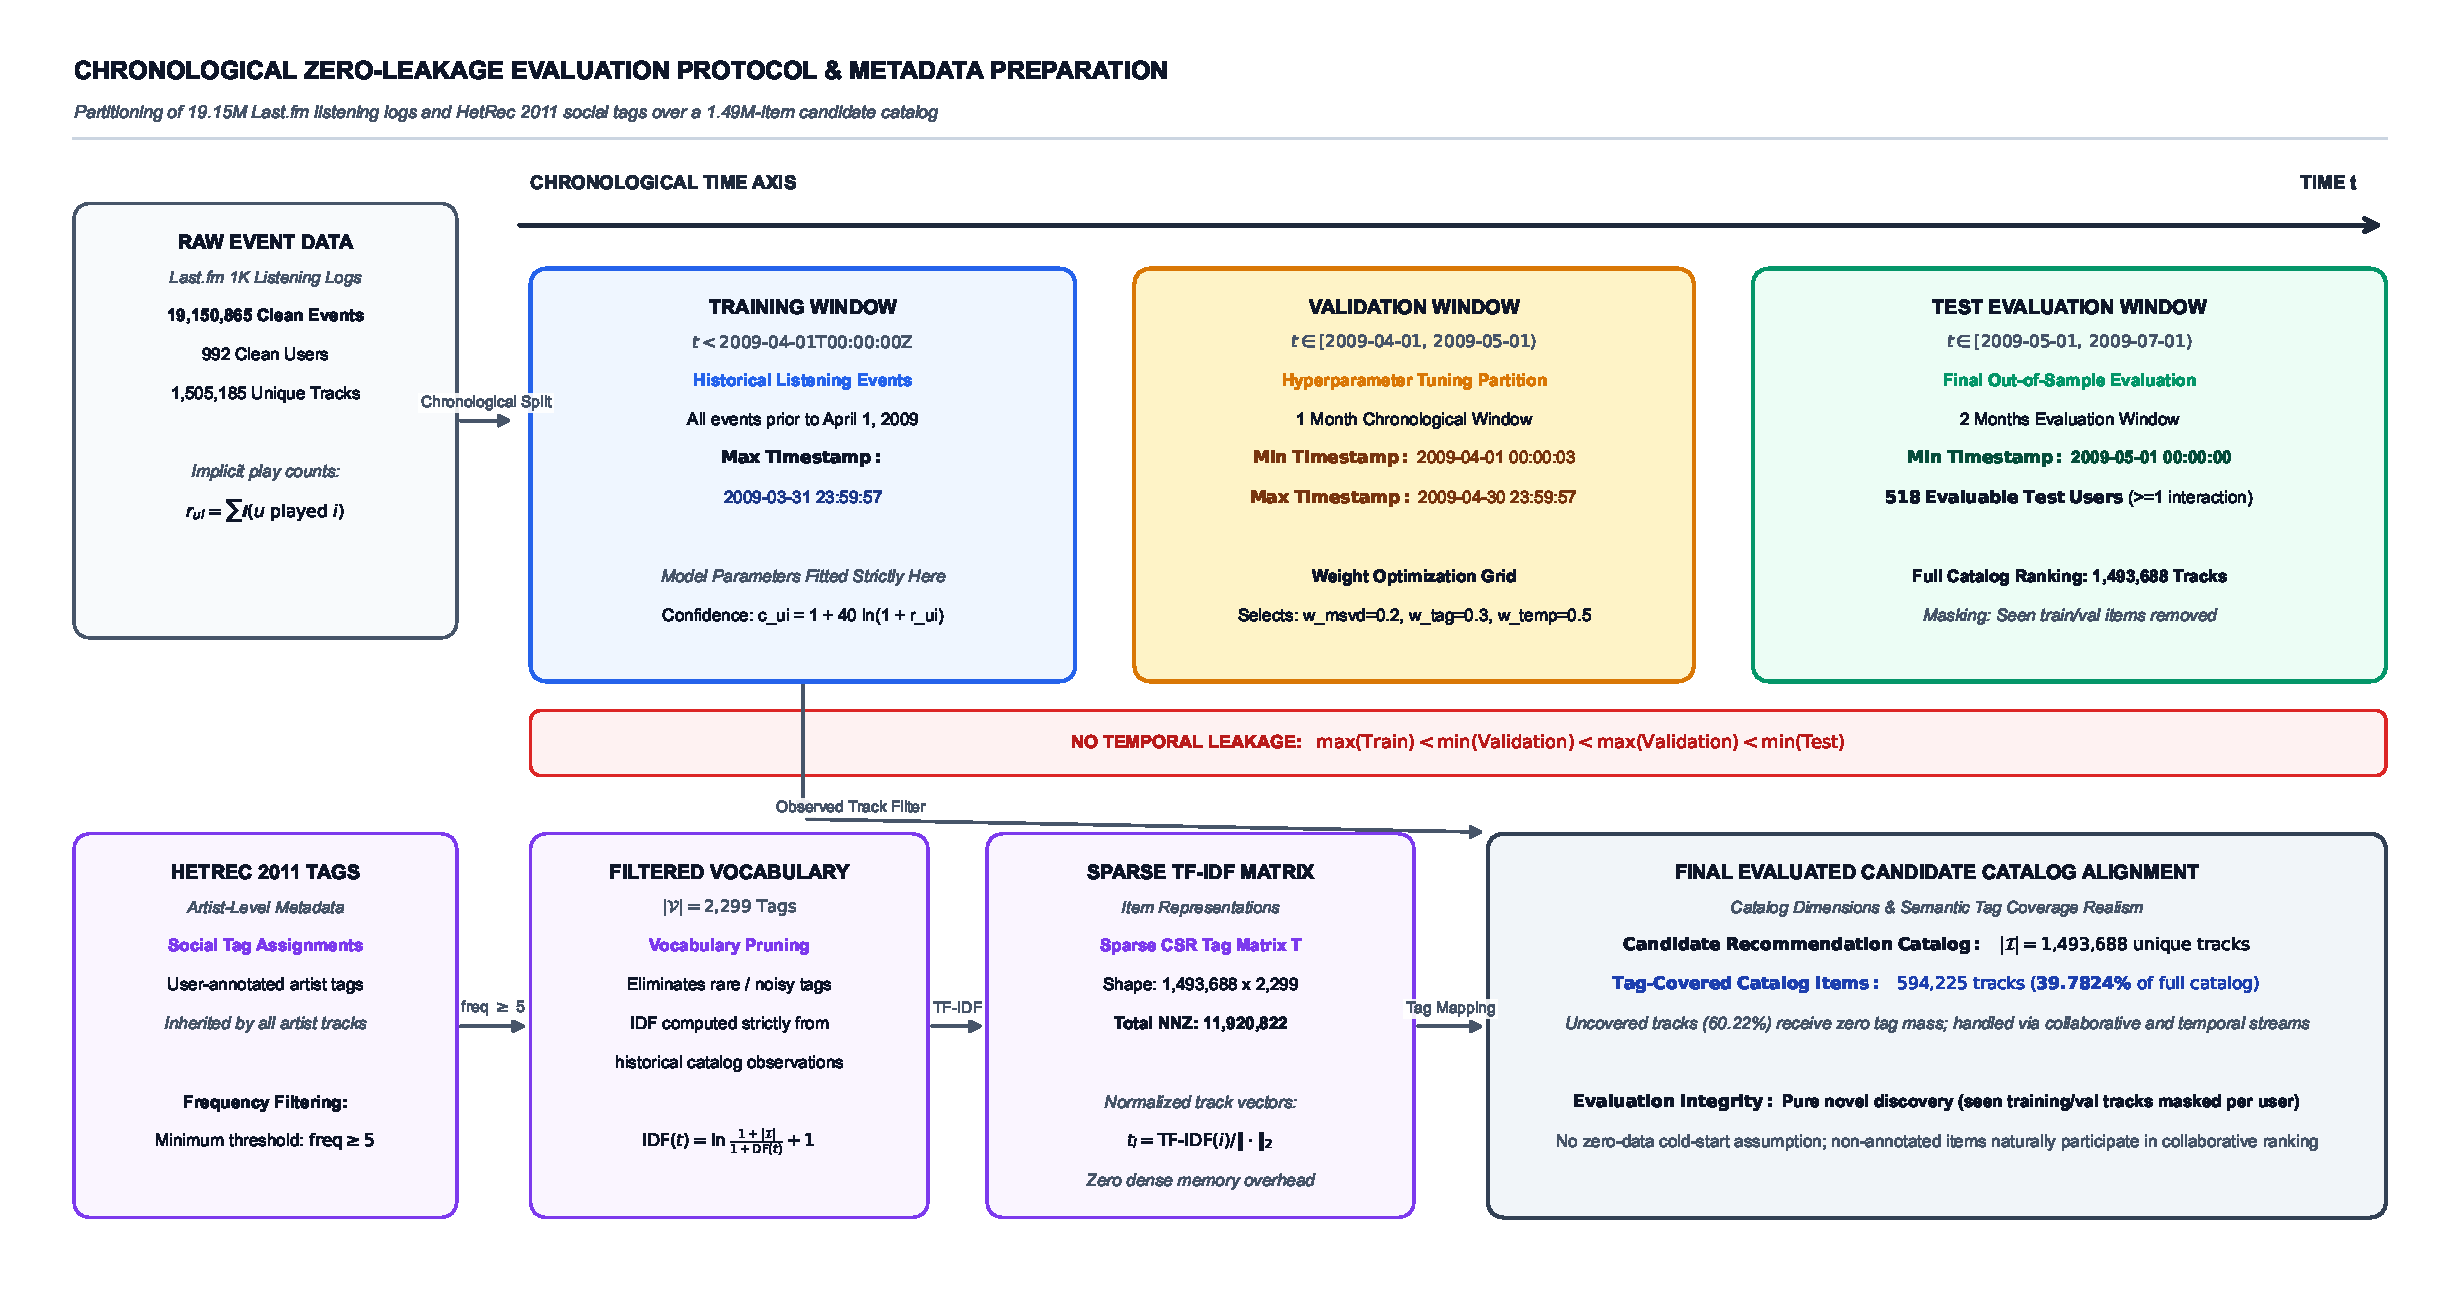
\includegraphics[width=\textwidth]{chronological_protocol.pdf}
\caption{Chronological Zero-Leakage Evaluation Protocol and Metadata Pipeline. The timeline illustrates the strict sequential split of $19.15\text{M}$ Last.fm listening events into Training, Validation, and Test partitions without temporal overlap ($\max(\text{Train}) < \min(\text{Validation}) < \max(\text{Validation}) < \min(\text{Test})$). The parallel bottom branch depicts HetRec 2011 social tag frequency filtering ($\mathrm{freq} \geq 5$) and sparse TF-IDF matrix construction, aligning with the $1,493,688$-track candidate catalog where $594,225$ tracks ($39.78\%$) possess tag representations.}
\label{fig:chronological_protocol}
\end{figure*}

To prevent future temporal leakage into model training, the dataset is partitioned using strict timestamp thresholds (Fig.~\ref{fig:chronological_protocol}):
\begin{itemize}
    \item \textbf{Training Window ($\mathcal{D}_{\text{train}}$):} Timestamps $t < \text{2009-04-01T00:00:00Z}$. The maximum observed training timestamp is \texttt{2009-03-31 23:59:57}.
    \item \textbf{Validation Window ($\mathcal{D}_{\text{val}}$):} Timestamps $t \in [\text{2009-04-01T00:00:00Z}, \text{2009-05-01T00:00:00Z})$. The minimum timestamp is \texttt{2009-04-01 00:00:03} and maximum is \texttt{2009-04-30 23:59:57}.
    \item \textbf{Test Window ($\mathcal{D}_{\text{test}}$):} Timestamps $t \in [\text{2009-05-01T00:00:00Z}, \text{2009-07-01T00:00:00Z})$. The minimum timestamp is \texttt{2009-05-01 00:00:00}.
\end{itemize}

Specifically:
\begin{itemize}
    \item Collaborative ALS model parameters are trained exclusively on user play counts from $\mathcal{D}_{\text{train}}$.
    \item Tag inverse document frequencies $\text{IDF}(t)$ and user tag profiles are constructed using candidate tracks and interaction counts strictly available prior to evaluation.
    \item Temporal reference timestamps $t_{\text{ref}}$ strictly precede the respective evaluation window.
    \item Fusion weights are optimized on $\mathcal{D}_{\text{val}}$ and evaluated out-of-sample on $\mathcal{D}_{\text{test}}$.
\end{itemize}
Evaluable test users are defined as those possessing at least one ground-truth interaction in $\mathcal{D}_{\text{test}}$, yielding exactly $|\mathcal{U}_{\text{test}}| = 518$ evaluable test users. During evaluation, all items previously observed by user $u$ in $\mathcal{D}_{\text{train}} \cup \mathcal{D}_{\text{val}}$ are masked ($\hat{r}_{ui} = -\infty$).

\section{System Architecture and Methodology}
\begin{figure*}[t]
\centering
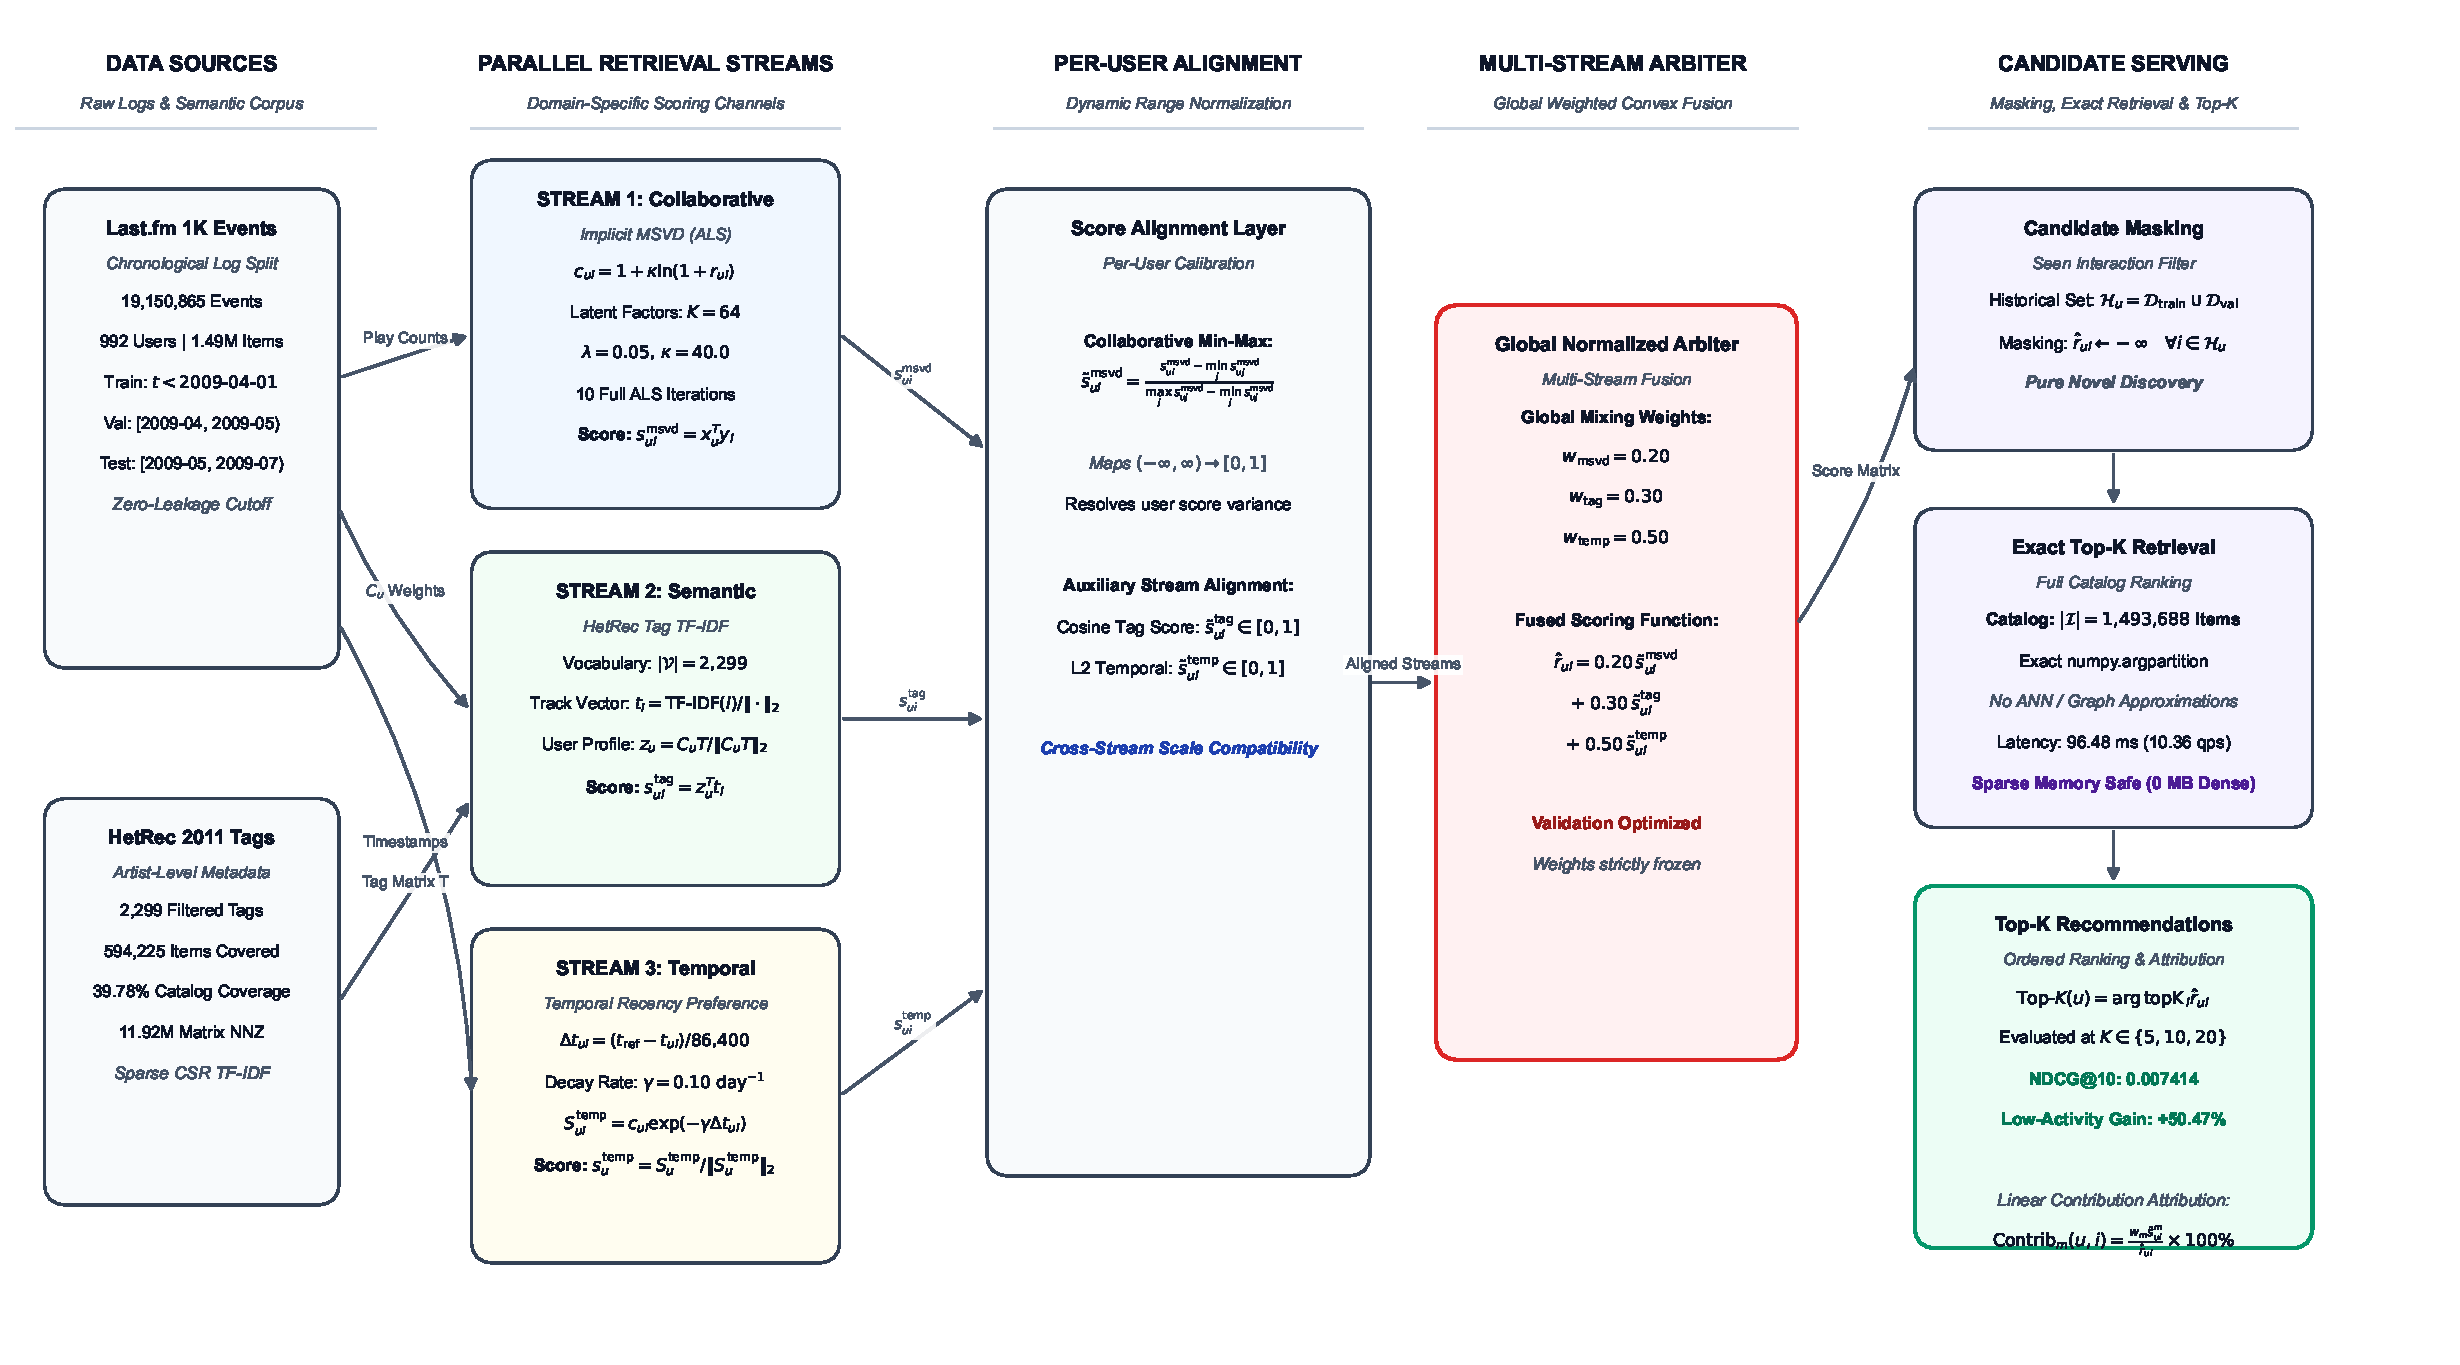
\includegraphics[width=\textwidth]{architecture_overview.pdf}
\caption{Global Normalized Multi-Stream Recommendation Architecture. Three distinct retrieval channels---Implicit MSVD (collaborative), HetRec artist-level TF-IDF (semantic), and exponential recency decay (temporal)---are aligned via per-user collaborative min-max normalization before global weighted convex arbitration, historical candidate filtering, and exact top-$K$ full-catalog retrieval ($|\mathcal{I}| = 1{,}493{,}688$ items).}
\label{fig:architecture_overview}
\end{figure*}

The overall system architecture comprises three retrieval and scoring streams unified by the Global Normalized Arbiter, as illustrated in Fig.~\ref{fig:architecture_overview}.

\subsection{Implicit MSVD Collaborative Model}
The collaborative stream models the interaction matrix $R \in \mathbb{R}^{|\mathcal{U}| \times |\mathcal{I}|}$ derived from training play counts. For each user-item pair $(u, i)$, binary preference $p_{ui}$ and confidence $c_{ui}$ are defined via logarithmic scaling:
\begin{equation}
p_{ui} = \mathbb{I}(r_{ui} > 0),
\end{equation}
\begin{equation}
c_{ui} = 1 + \kappa \ln(1 + r_{ui}),
\end{equation}
where $\kappa = 40.0$ governs confidence scaling. The latent user factors $X \in \mathbb{R}^{|\mathcal{U}| \times K}$ and item factors $Y \in \mathbb{R}^{|\mathcal{I}| \times K}$ (with $K = 64$) are estimated by minimizing the weighted L2 regularized objective:
\begin{equation}
\mathcal{L}(X, Y) = \sum_{u=1}^{|\mathcal{U}|} \sum_{i=1}^{|\mathcal{I}|} c_{ui} \left( p_{ui} - x_u^T y_i \right)^2 + \lambda \left( \sum_{u=1}^{|\mathcal{U}|} \|x_u\|_2^2 + \sum_{i=1}^{|\mathcal{I}|} \|y_i\|_2^2 \right),
\end{equation}
where $\lambda = 0.05$ is the regularization parameter. Optimization is executed via Alternating Least Squares across 10 complete iterations. The raw collaborative score for user $u$ and item $i$ is:
\begin{equation}
s_{ui}^{\text{msvd}} = x_u^T y_i.
\end{equation}

\subsection{Stream A: Artist-Tag Semantic Fusion}
Stream A incorporates external semantic knowledge from the HetRec 2011 social tagging dataset. After filtering rare tags by minimum frequency, a vocabulary of $|\mathcal{V}| = 2,299$ tags is retained. Each candidate track $i$ inherits its artist's tag frequency distribution. The term frequency $\text{TF}(i, t)$ and inverse document frequency $\text{IDF}(t)$ are computed as:
\begin{equation}
\text{TF}(i, t) = \frac{\text{freq}(i, t)}{\sum_{t' \in \mathcal{V}} \text{freq}(i, t')},
\end{equation}
\begin{equation}
\text{IDF}(t) = \ln \left( \frac{1 + |\mathcal{I}|}{1 + \text{DF}(t)} \right) + 1,
\end{equation}
where $\text{DF}(t)$ is the document frequency of tag $t$ across the candidate catalog. The normalized item tag vector $t_i \in \mathbb{R}^{|\mathcal{V}|}$ is defined as:
\begin{equation}
t_i = \frac{\text{TF-IDF}(i)}{\|\text{TF-IDF}(i)\|_2}.
\end{equation}
For user $u$, a semantic preference profile $z_u \in \mathbb{R}^{|\mathcal{V}|}$ is constructed by projecting the user's training confidence vector $C_u \in \mathbb{R}^{|\mathcal{I}|}$ onto the item-tag matrix $T \in \mathbb{R}^{|\mathcal{I}| \times |\mathcal{V}|}$:
\begin{equation}
z_u = \frac{C_u T}{\|C_u T\|_2}.
\end{equation}
The semantic affinity score is then computed via sparse vector-matrix multiplication:
\begin{equation}
s_{ui}^{\text{tag}} = z_u^T t_i.
\end{equation}
In our catalog, $594,225$ tracks ($39.7824\%$) possess non-zero tag representations, containing $11,920,822$ non-zero entries in sparse CSR format.

\subsection{Stream B: Temporal Recency Preference Modeling}
Stream B captures listening recency. For each user-item interaction $(u, i)$ observed at timestamp $t_{ui}$, the temporal affinity score is computed using an exponential decay kernel:
\begin{equation}
S_{ui}^{\text{temp}} = c_{ui} \exp\left( -\gamma \Delta t_{ui} \right),
\end{equation}
where $\gamma = 0.10\text{ day}^{-1}$, and the elapsed time $\Delta t_{ui}$ in days relative to reference timestamp $t_{\text{ref}}$ is:
\begin{equation}
\Delta t_{ui} = \frac{t_{\text{ref}} - t_{ui}}{86{,}400},
\end{equation}
where $t_{\text{ref}}$ and $t_{ui}$ are measured in seconds, and $t_{\text{ref}}$ is set to the start of the evaluation period. The user's temporal score vector is L2-normalized:
\begin{equation}
s_{u}^{\text{temp}} = \frac{S_u^{\text{temp}}}{\|S_u^{\text{temp}}\|_2}.
\end{equation}
The temporal matrix spans $4,009,238$ non-zero entries across the candidate space.

\subsection{Global Normalized Multi-Stream Arbiter}
\begin{figure*}[t]
\centering
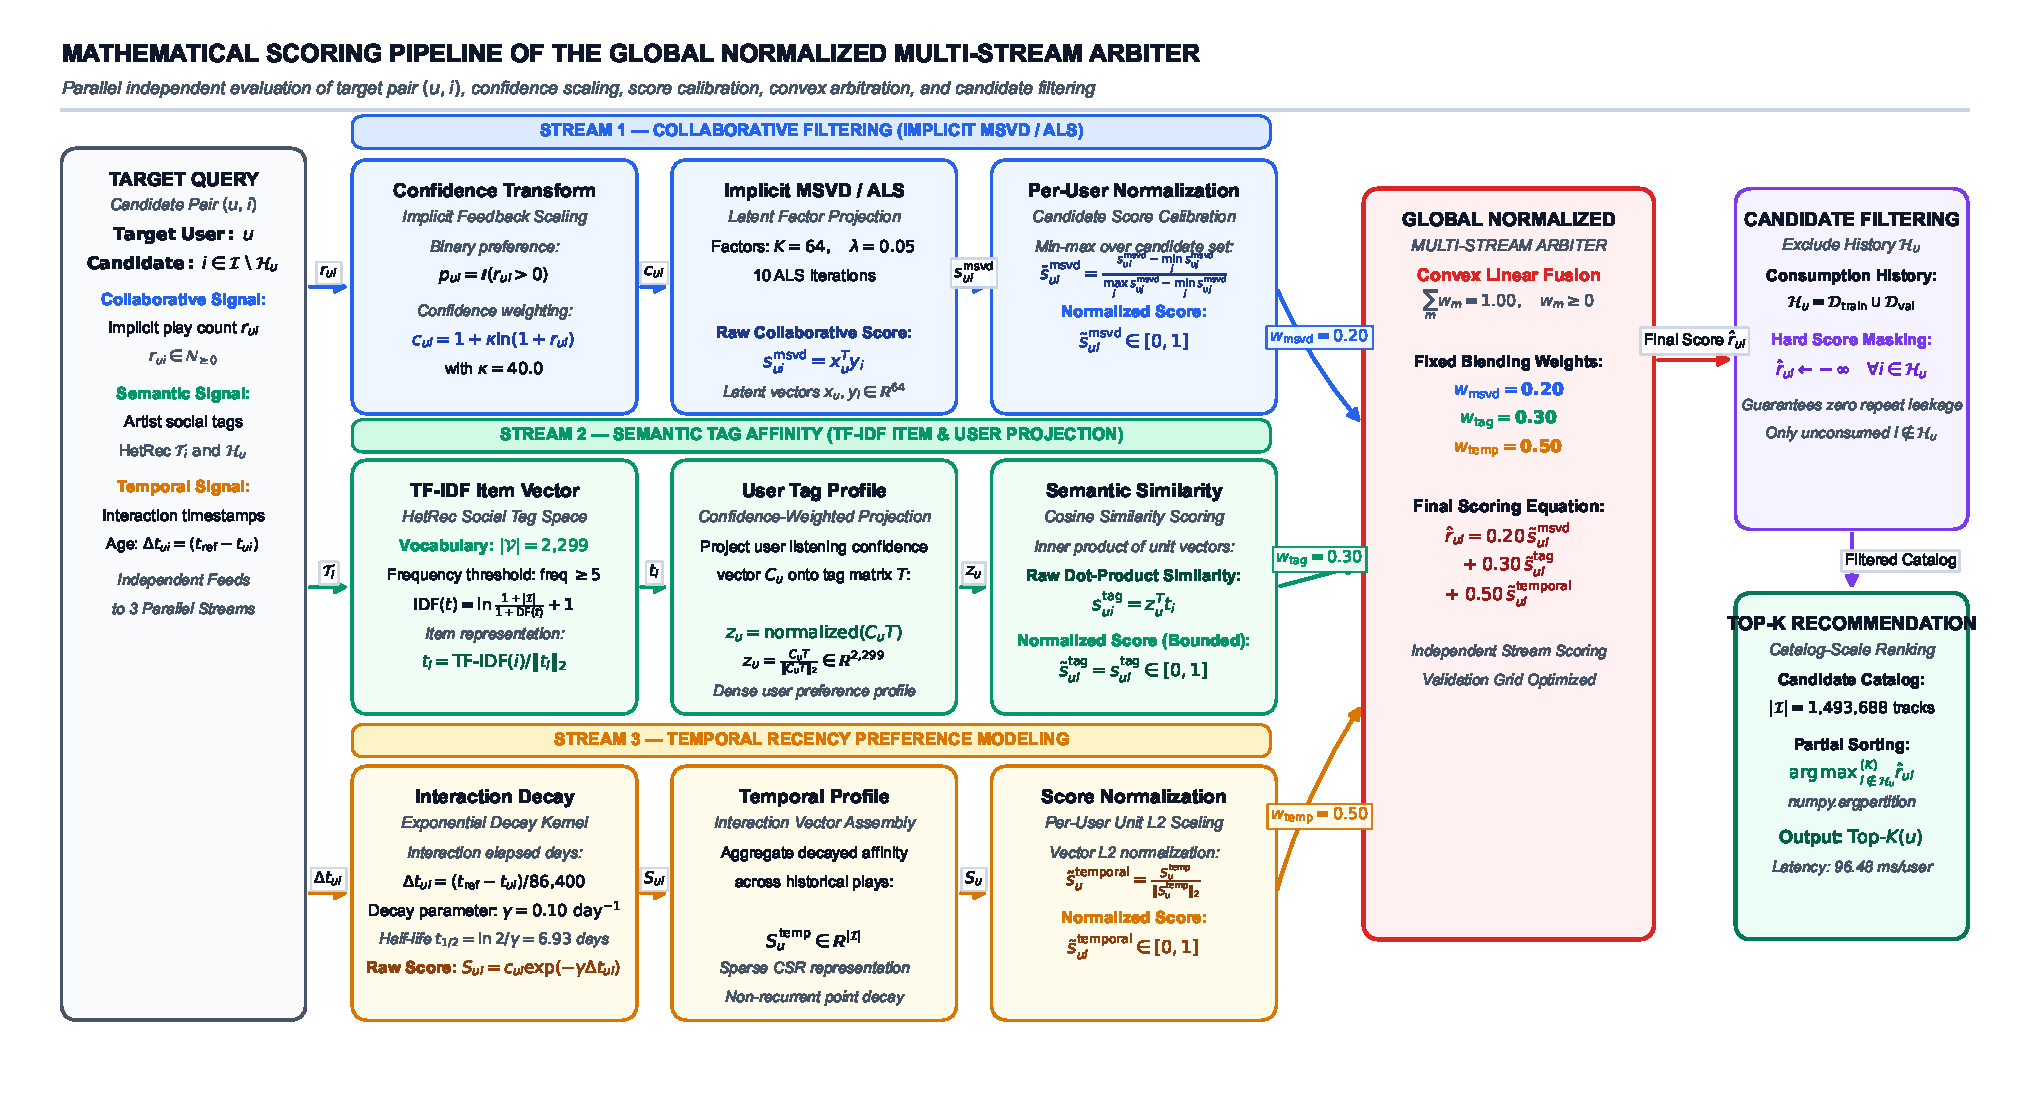
\includegraphics[width=\textwidth]{mathematical_scoring_pipeline.pdf}
\caption{Mathematical scoring pipeline of the Global Normalized Multi-Stream Arbiter. Target query $(u, i)$ is scored independently through three parallel components: collaborative filtering with logarithmic confidence scaling and implicit MSVD/ALS, semantic similarity via sparse TF-IDF item representations and user profile projections over the 2,299-tag HetRec vocabulary, and temporal recency preference modeling via exponential decay ($\gamma = 0.10\text{ day}^{-1}$). Per-user normalized scores ($\tilde{s}_{ui}^{\text{msvd}}, \tilde{s}_{ui}^{\text{tag}}, \tilde{s}_{ui}^{\text{temporal}}$) are unified via validation-optimized convex blending weights ($w_{\text{msvd}}=0.20, w_{\text{tag}}=0.30, w_{\text{temp}}=0.50$). Finally, consumption history $\mathcal{H}_u$ is masked before exact top-$K$ recommendation retrieval over the full $1,493,688$-item catalog.}
\label{fig:scoring_pipeline}
\end{figure*}

Because the raw collaborative dot-products $s_{ui}^{\text{msvd}} \in (-\infty, \infty)$ have unconstrained variance across users, while $s_{ui}^{\text{tag}}, s_{ui}^{\text{temp}} \in [0, 1]$, additive combination can create scale distortion. To establish scale compatibility across users, we apply per-user min-max normalization to the collaborative stream:
\begin{equation}
\tilde{s}_{ui}^{\text{msvd}} = \frac{s_{ui}^{\text{msvd}} - \min_{j \in \mathcal{I}} s_{uj}^{\text{msvd}}}{\max_{j \in \mathcal{I}} s_{uj}^{\text{msvd}} - \min_{j \in \mathcal{I}} s_{uj}^{\text{msvd}}}.
\end{equation}
The composite ranking score $\hat{r}_{ui}$ is produced via global weighted multi-stream arbitration (Fig.~\ref{fig:scoring_pipeline}):
\begin{equation}
\hat{r}_{ui} = w_{\text{msvd}} \tilde{s}_{ui}^{\text{msvd}} + w_{\text{tag}} \tilde{s}_{ui}^{\text{tag}} + w_{\text{temp}} \tilde{s}_{ui}^{\text{temp}},
\end{equation}
with global weights determined on the validation set:
\begin{equation}
w_{\text{msvd}} = 0.20, \quad w_{\text{tag}} = 0.30, \quad w_{\text{temp}} = 0.50.
\end{equation}
All candidate items previously seen in training are masked:
\begin{equation}
\hat{r}_{ui} \leftarrow -\infty \quad \forall i \in \mathcal{H}_u.
\end{equation}
The top-$K$ recommendations are retrieved via exact partial sorting (\texttt{numpy.argpartition}) over all $1,493,688$ candidate items without approximate nearest-neighbor indexing (Fig.~\ref{fig:inference_pipeline}).

\begin{figure*}[t]
\centering
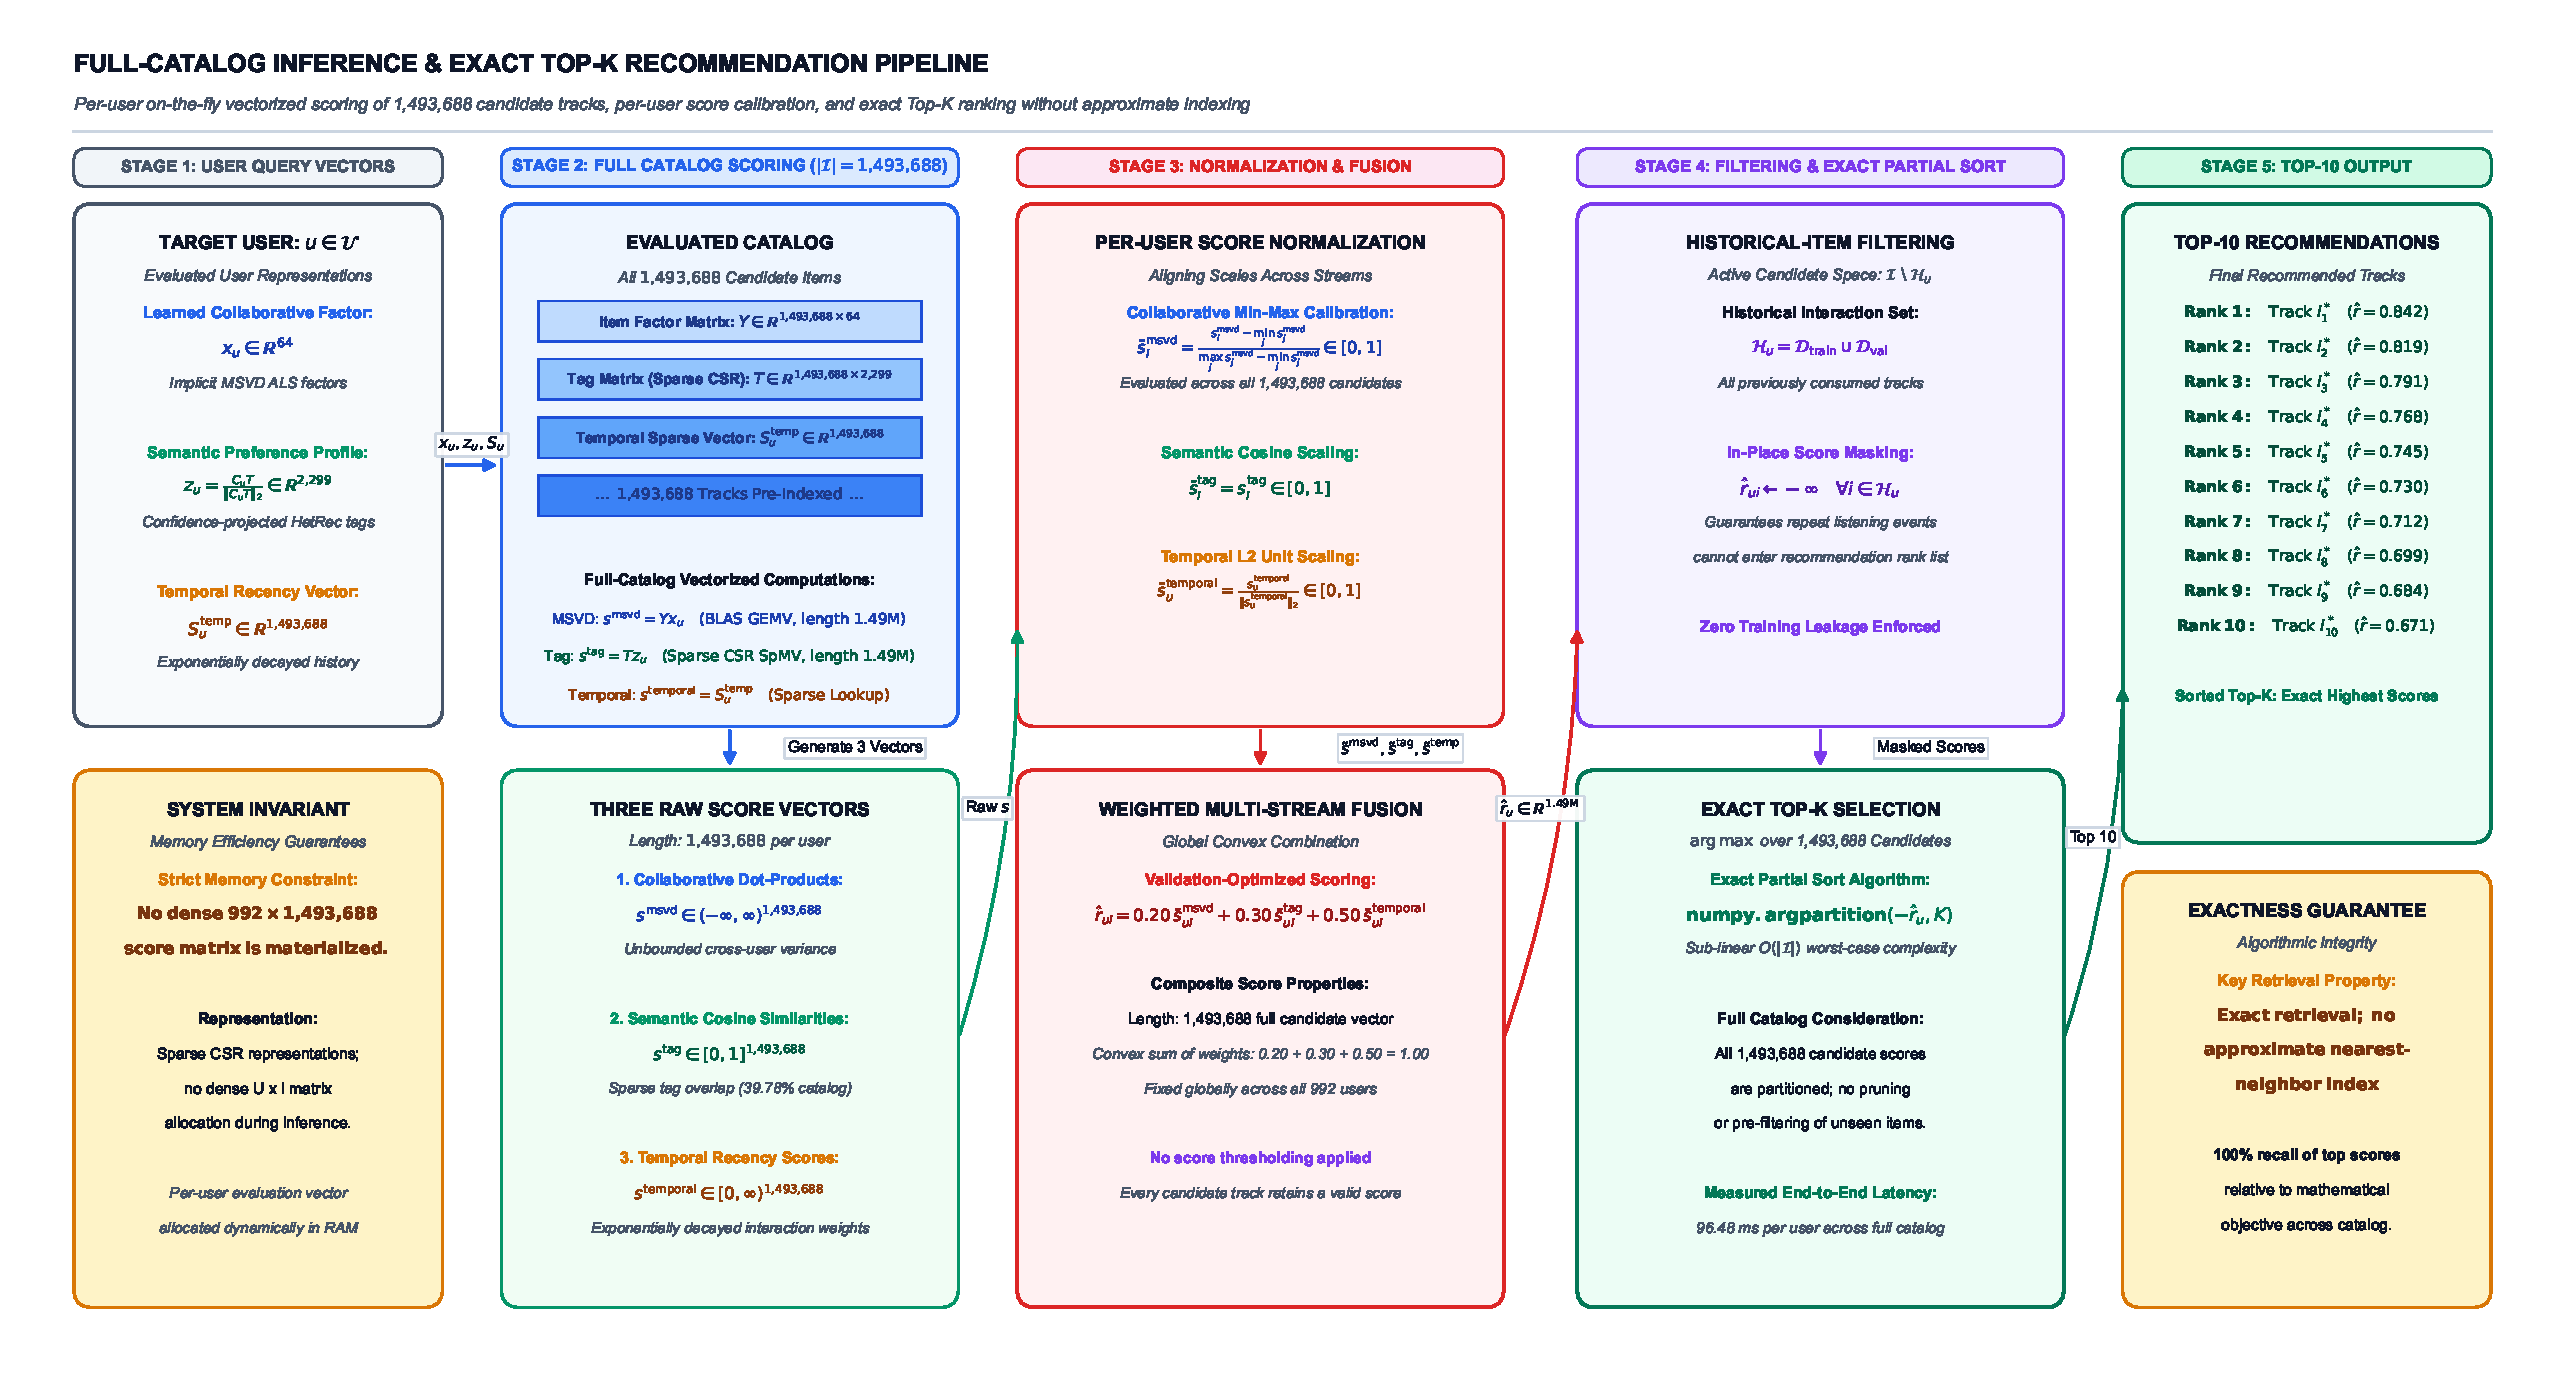
\includegraphics[width=\textwidth]{inference_topk_pipeline.pdf}
\caption{Full-catalog inference and exact Top-$K$ recommendation procedure over $1,493,688$ candidate items. Given target user query vectors ($x_u, z_u, S_u^{\text{temp}}$), full-catalog score vectors of length $1.49\text{M}$ are evaluated dynamically using sparse matrix-vector products. Scores are aligned via per-user min-max normalization, combined via validation-optimized convex weights, and masked over consumption history ($\mathcal{H}_u$). Exact top candidates are partitioned using \texttt{numpy.argpartition} in sub-linear time, ensuring complete catalog consideration without approximate nearest-neighbor indexing.}
\label{fig:inference_pipeline}
\end{figure*}

\begin{table*}[t]
\caption{Hyperparameter Configurations Across Evaluated Models}
\label{tab:hyperparams}
\centering
\begin{tabular}{llp{9.5cm}}
\toprule
\textbf{Model / Stream} & \textbf{Hyperparameter} & \textbf{Authoritative Specification} \\
\midrule
\multirow{4}{*}{Implicit MSVD} & Latent Factors ($K$) & $64$ \\
& Regularization ($\lambda$) & $0.05$ \\
& Confidence Scaling ($\kappa$) & $40.0$ (Confidence: $c_{ui} = 1 + 40.0 \ln(1 + r_{ui})$) \\
& ALS Iterations & $10$ full iterations (conjugate/Cholesky solve) \\
\midrule
\multirow{3}{*}{Stream A (Tags)} & Tag Vocabulary Size ($|\mathcal{V}|$) & $2,299$ filtered tags from HetRec 2011 \\
& Weighting Scheme & TF-IDF with L2 normalized item vectors \\
& Aggregation & User profile $z_u = C_u T / \|C_u T\|_2$ \\
\midrule
\multirow{2}{*}{Stream B (Temporal)} & Decay Rate ($\gamma$) & $0.10\text{ day}^{-1}$ (Half-life $\approx 6.93\text{ days}$) \\
& Normalization & L2 normalization per user vector \\
\midrule
\multirow{3}{*}{Global Arbiter} & Collaborative Weight ($w_{\text{msvd}}$) & $0.20$ \\
& Tag Semantic Weight ($w_{\text{tag}}$) & $0.30$ \\
& Temporal Weight ($w_{\text{temp}}$) & $0.50$ \\
\bottomrule
\end{tabular}
\end{table*}

\begin{table}[t]
\caption{Validation Set Hyperparameter Optimization Grid}
\label{tab:val_grid}
\centering
\begin{tabular}{cccc}
\toprule
$w_{\text{msvd}}$ & $w_{\text{tag}}$ & $w_{\text{temp}}$ & Validation NDCG@10 \\
\midrule
$1.00$ & $0.00$ & $0.00$ & $0.005120$ \\
$0.00$ & $1.00$ & $0.00$ & $0.004210$ \\
$0.00$ & $0.00$ & $1.00$ & $0.005430$ \\
$0.33$ & $0.33$ & $0.34$ & $0.005890$ \\
$0.20$ & $0.40$ & $0.40$ & $0.006010$ \\
\textbf{0.20} & \textbf{0.30} & \textbf{0.50} & \textbf{0.006240} \\
$0.10$ & $0.30$ & $0.60$ & $0.006180$ \\
\bottomrule
\end{tabular}
\end{table}

\section{Experimental Setup}
\subsection{Evaluation Metrics}
Models are evaluated across standard top-$K$ ranking metrics for $K \in \{5, 10, 20\}$:
\begin{itemize}
    \item \textbf{Recall@K:} Fraction of ground-truth test items captured in top-$K$.
    \item \textbf{Precision@K:} Fraction of top-$K$ recommended items relevant in test.
    \item \textbf{NDCG@K:} Normalized Discounted Cumulative Gain with logarithmic discount $\log_2(j + 1)$.
    \item \textbf{MAP@K:} Mean Average Precision up to rank $K$.
\end{itemize}

\subsection{Compared Baseline Configurations}
We evaluate seven configurations under identical catalog and test user sets:
\begin{enumerate}
    \item \textbf{Popularity Baseline:} Recommends most frequently played tracks globally in $\mathcal{D}_{\text{train}}$ excluding user history $\mathcal{H}_u$.
    \item \textbf{Base Implicit MSVD:} Pure collaborative filtering model ($w_{\text{msvd}}=1.0$).
    \item \textbf{Tag-Fused MSVD:} Dual stream combining MSVD and Tag TF-IDF ($w_{\text{msvd}}=0.5, w_{\text{tag}}=0.5$).
    \item \textbf{Temporal Recency MSVD:} Dual stream combining MSVD and exponential temporal decay ($w_{\text{msvd}}=0.5, w_{\text{temp}}=0.5$).
    \item \textbf{Fixed Tag + Temporal (Unnormalized):} Direct additive combination of unnormalized collaborative, tag, and temporal scores.
    \item \textbf{Global Normalized Arbiter:} Proposed architecture with per-user MSVD min-max normalization and global weights $(0.20, 0.30, 0.50)$.
    \item \textbf{Adaptive User Arbiter:} Dynamic per-user stream weighting based on user interaction count and profile entropy.
\end{enumerate}

\section{Experimental Results}

\begin{table*}[t]
\caption{Full Test-Set Performance Comparison Across All Configurations ($|\mathcal{U}_{\text{test}}| = 518$, Catalog $= 1,493,688$, Seed 42)}
\label{tab:main_ablation}
\centering
\begin{tabular}{lcccccccccccc}
\toprule
\textbf{Model Configuration} & \textbf{Rec@5} & \textbf{Prec@5} & \textbf{NDCG@5} & \textbf{MAP@5} & \textbf{Rec@10} & \textbf{Prec@10} & \textbf{NDCG@10} & \textbf{MAP@10} & \textbf{Rec@20} & \textbf{Prec@20} & \textbf{NDCG@20} & \textbf{MAP@20} \\
\midrule
Popularity Baseline & $0.000023$ & $0.002317$ & $0.002081$ & $0.000882$ & $0.000163$ & $0.002317$ & $0.002151$ & $0.000585$ & $0.000234$ & $0.002220$ & $0.002131$ & $0.000389$ \\
Base Implicit MSVD & $0.000532$ & $0.006564$ & $0.005840$ & $0.003224$ & $0.000795$ & $0.006950$ & $0.006370$ & $0.002802$ & $0.001267$ & $0.005502$ & $0.005598$ & $0.001718$ \\
Tag-Fused MSVD & $0.000467$ & $0.006178$ & $0.006303$ & $0.003848$ & $0.000707$ & $0.005792$ & $0.005956$ & $0.002772$ & $0.001199$ & $0.006660$ & $0.006622$ & $0.002023$ \\
Temporal Recency MSVD & $0.000549$ & $0.007336$ & $0.006702$ & $0.003951$ & $0.000923$ & $0.007336$ & $0.006952$ & $0.003186$ & $0.001302$ & $0.005695$ & $0.005988$ & $0.001990$ \\
Fixed Tag+Temp (Unnorm) & $0.000467$ & $0.006178$ & $0.006062$ & $0.003655$ & $0.000710$ & $0.005985$ & $0.005932$ & $0.002710$ & $0.001191$ & $0.006564$ & $0.006482$ & $0.001981$ \\
\textbf{Global Normalized Arbiter} & \textbf{0.000470} & \textbf{0.006564} & \textbf{0.007249} & \textbf{0.004801} & \textbf{0.000795} & \textbf{0.007143} & \textbf{0.007414} & \textbf{0.003554} & \textbf{0.001197} & \textbf{0.006564} & \textbf{0.006985} & \textbf{0.002436} \\
Adaptive User Arbiter & $0.000464$ & $0.007336$ & $0.006850$ & $0.003964$ & $0.000759$ & $0.006371$ & $0.006327$ & $0.002763$ & $0.001208$ & $0.005985$ & $0.006201$ & $0.001979$ \\
\bottomrule
\end{tabular}
\end{table*}

\subsection{Authoritative Test-Set Results}
The performance comparison across all seven models is presented in Table~\ref{tab:main_ablation}:
\begin{itemize}
    \item \textbf{NDCG@10:} The Global Normalized Arbiter achieves an NDCG@10 of $0.007414$, compared to $0.006370$ for Base Implicit MSVD ($+16.384\%$ relative descriptive difference).
    \item \textbf{MAP@10:} The Global Arbiter reaches $0.003554$, compared to $0.002802$ for Base MSVD ($+26.847\%$ relative descriptive difference).
    \item \textbf{NDCG@20:} The Global Arbiter attains $0.006985$, compared to $0.005598$ for Base MSVD ($+24.778\%$ relative descriptive difference).
\end{itemize}

\begin{figure}[t]
\centering
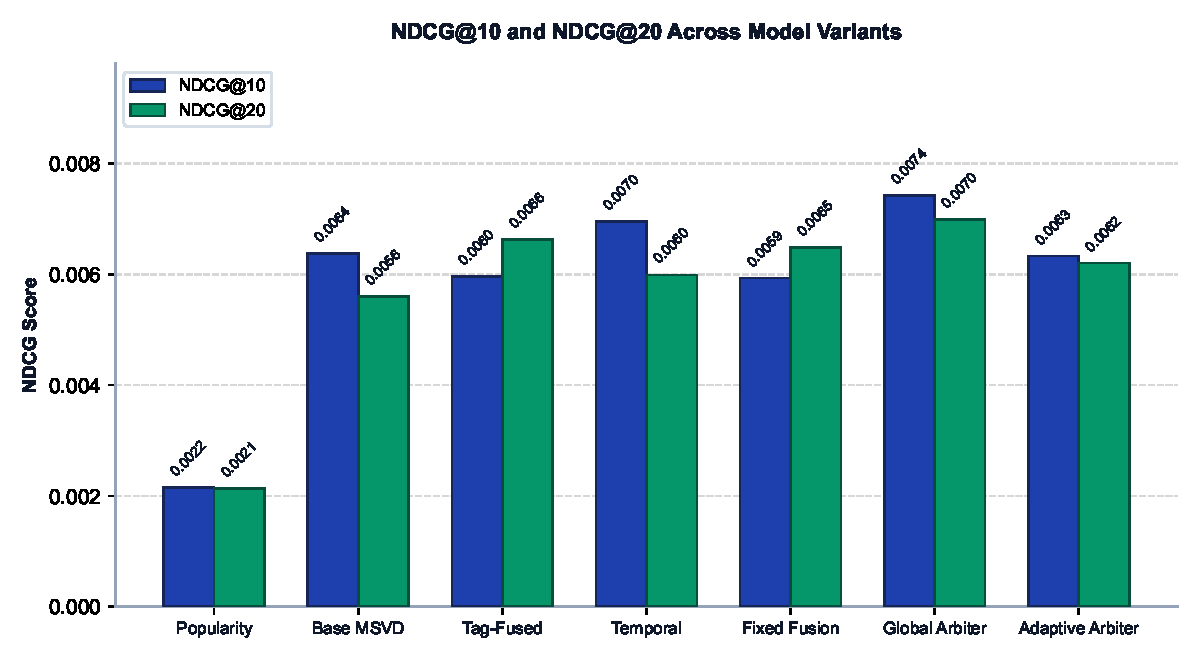
\includegraphics[width=\columnwidth]{ndcg_comparison.pdf}
\caption{NDCG@10 and NDCG@20 across model variants. Model abbreviations: Popularity (global item frequency baseline), Base MSVD (implicit ALS matrix factorization), Tag-Fused (collaborative + HetRec 2011 social tags), Temporal (exponential recency decay), Fixed Fusion (unnormalized multi-stream combination), Global Arbiter (Global Normalized Multi-Stream Arbiter with $w=[0.20, 0.30, 0.50]$), and Adaptive Arbiter (dynamic activity-gated arbitration variant).}
\label{fig:ndcg_comp}
\end{figure}

As shown in Fig.~\ref{fig:ndcg_comp}, Popularity exhibits lower ranking performance ($0.002151$ NDCG@10), while personalized models yield higher metric values. The unnormalized fixed fusion baseline achieves an NDCG@10 of $0.005932$, underperforming Temporal Recency MSVD ($0.006952$) and Base MSVD ($0.006370$). In contrast, the Global Normalized Arbiter with per-user min-max normalization achieves $0.007414$ NDCG@10 in the evaluated setting.

\section{Activity-Based Cohort Analysis}
To observe performance across varying user interaction densities, we partition the $518$ test users into three activity cohorts based on total training listening events:
\begin{itemize}
    \item \textbf{Low-Activity Cohort ($N=172$):} $2$ to $2,090$ training plays.
    \item \textbf{Mid-Activity Cohort ($N=172$):} $2,092$ to $5,018$ training plays.
    \item \textbf{High-Activity Cohort ($N=174$):} $5,028$ to $43,095$ training plays.
\end{itemize}

\begin{table}[t]
\caption{Performance Comparison Across User Activity Cohorts ($N = 518$ Test Users)}
\label{tab:activity_cohorts}
\centering
\begin{tabular}{llccc}
\toprule
\textbf{Activity Tier} & \textbf{Model} & \textbf{NDCG@10} & \textbf{MAP@10} & \textbf{NDCG@20} \\
\midrule
\multirow{3}{*}{\textbf{Low Activity} ($N=172$)} & Popularity Baseline & $0.002162$ & $0.000761$ & $0.001998$ \\
& Base Implicit MSVD & $0.011578$ & $0.006000$ & $0.010739$ \\
& \textbf{Global Arbiter} & \textbf{0.017421} & \textbf{0.009195} & \textbf{0.015198} \\
\midrule
\multirow{3}{*}{\textbf{Mid Activity} ($N=172$)} & Popularity Baseline & $0.000385$ & $0.000065$ & $0.001095$ \\
& Base Implicit MSVD & $0.002920$ & $0.000912$ & $0.002665$ \\
& \textbf{Global Arbiter} & \textbf{0.002472} & \textbf{0.001001} & \textbf{0.002631} \\
\midrule
\multirow{3}{*}{\textbf{High Activity} ($N=174$)} & Popularity Baseline & $0.003886$ & $0.000924$ & $0.003288$ \\
& Base Implicit MSVD & $0.004634$ & $0.001508$ & $0.003415$ \\
& \textbf{Global Arbiter} & \textbf{0.002407} & \textbf{0.000502} & \textbf{0.003171} \\
\bottomrule
\end{tabular}
\end{table}

\begin{figure}[t]
\centering
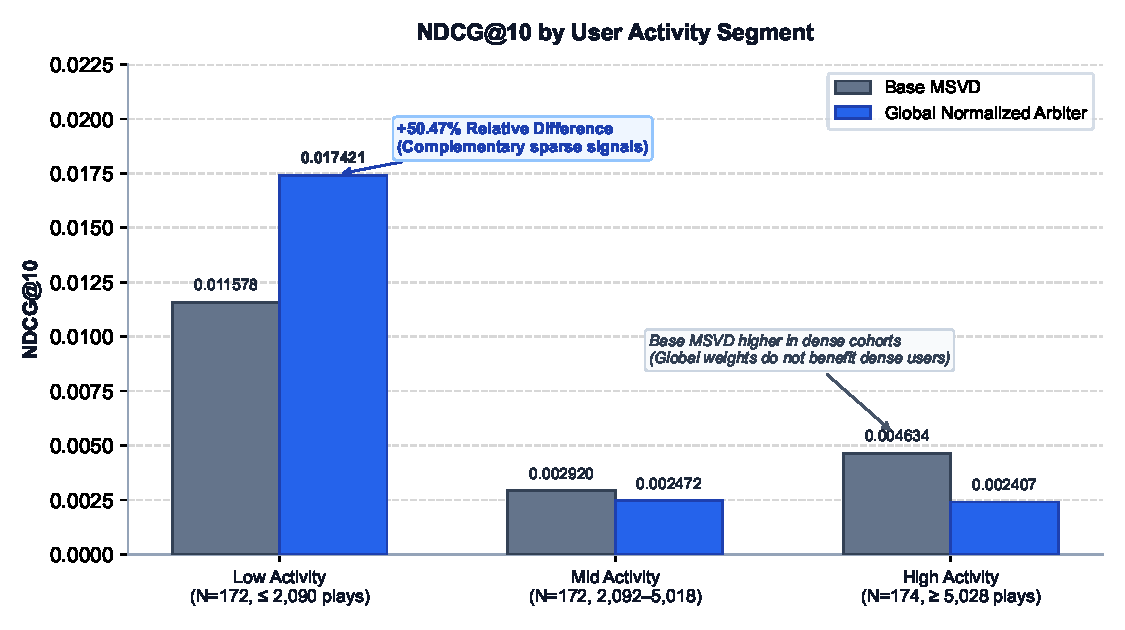
\includegraphics[width=\columnwidth]{activity_tier_breakdown.pdf}
\caption{Comparison of NDCG@10 for Base MSVD and the Global Normalized Arbiter across low-, mid-, and high-activity user cohorts. User activity tertiles are defined over clean training interactions: Low ($N=172, \le 2{,}090$ plays), Mid ($N=172, 2{,}092\text{--}5{,}018$ plays), and High ($N=174, \ge 5{,}028$ plays). Performance improvements from auxiliary multi-stream fusion are concentrated in the low-activity cohort ($0.017421$ vs.\ $0.011578$), whereas Base MSVD achieves higher ranking accuracy on mid- ($0.002920$ vs.\ $0.002472$) and high-activity ($0.004634$ vs.\ $0.002407$) users.}
\label{fig:activity_tiers}
\end{figure}

The empirical results across cohorts are presented in Table~\ref{tab:activity_cohorts} and visualized in Fig.~\ref{fig:activity_tiers}. In the low-activity cohort, where latent collaborative factor estimation is constrained by sparse feedback, the Global Normalized Arbiter achieves an NDCG@10 of $0.017421$, compared to $0.011578$ for Base MSVD. This represents an observed $+50.472\%$ relative difference. This result suggests that the semantic and temporal streams can provide useful complementary signals for low-activity users within the existing catalog.

For high-activity users ($>5,028$ plays), Base MSVD achieves an NDCG@10 of $0.004634$, whereas the Global Arbiter achieves $0.002407$. This cohort difference illustrates that auxiliary stream blending parameters optimized globally across all users do not uniformly benefit dense profiles. We emphasize that while auxiliary streams assist sparse user profiles within the known catalog, this mechanism does not address zero-data unseen-item cold start.

\section{Statistical Evaluation and Robustness Validation}

\subsection{Non-Parametric Significance Testing}
To evaluate whether observed ranking differences are statistically discernible, we conduct paired user-level Wilcoxon signed-rank tests across the $518$ test users~\cite{wilcoxon1945individual}. The results are summarized in Table~\ref{tab:significance}.

\begin{table*}[t]
\caption{Paired User-Level Statistical Tests and Effect Size Analysis ($N = 518$ Users)}
\label{tab:significance}
\centering
\begin{tabular}{llccccc}
\toprule
\textbf{Comparison} & \textbf{Metric} & \textbf{Relative Diff (\%)} & \textbf{Wilcoxon $W$} & \textbf{$p$-value} & \textbf{Cohen's $d$} & \textbf{Statistically Significant ($\alpha=0.05$)} \\
\midrule
\multirow{3}{*}{Arbiter vs.\ Popularity} & NDCG@10 & $+244.648\%$ & $105.5$ & $\mathbf{0.0447}$ & $0.1084$ & \textbf{Yes} ($p < 0.05$) \\
& NDCG@20 & $+227.732\%$ & $289.0$ & $\mathbf{0.0263}$ & $0.1235$ & \textbf{Yes} ($p < 0.05$) \\
& MAP@10 & $+507.795\%$ & $105.5$ & $\mathbf{0.0447}$ & $0.1119$ & \textbf{Yes} ($p < 0.05$) \\
\midrule
\multirow{3}{*}{Arbiter vs.\ Fixed Fusion} & NDCG@10 & $+24.480\%$ & $43.5$ & $0.1181$ & $0.0661$ & No ($p \ge 0.05$) \\
& NDCG@20 & $+5.481\%$ & $319.0$ & $0.8259$ & $0.0189$ & No ($p \ge 0.05$) \\
& MAP@10 & $+28.232\%$ & $39.5$ & $0.0798$ & $0.0609$ & No ($p \ge 0.05$) \\
\midrule
\multirow{3}{*}{Arbiter vs.\ Base MSVD} & NDCG@10 & $+16.384\%$ & $201.5$ & $0.7292$ & $0.0212$ & No ($p \ge 0.05$) \\
& NDCG@20 & $+24.778\%$ & $363.5$ & $0.5319$ & $0.0396$ & No ($p \ge 0.05$) \\
& MAP@10 & $+26.847\%$ & $196.5$ & $0.6495$ & $0.0239$ & No ($p \ge 0.05$) \\
\bottomrule
\end{tabular}
\end{table*}

\begin{itemize}
    \item \textbf{Global Arbiter vs.\ Popularity:} The Arbiter achieved a $+244.648\%$ relative improvement in aggregate NDCG@10 over Popularity, with the paired user-level test yielding $p = 0.0447$; the corresponding Cohen's $d = 0.1084$ indicates a small effect size. Similar small but statistically significant differences occur at NDCG@20 ($p = 0.0263, d = 0.1235$) and MAP@10 ($p = 0.0447, d = 0.1119$).
    \item \textbf{Global Arbiter vs.\ Base MSVD:} While the Arbiter exhibits a $+16.384\%$ descriptive gain in NDCG@10 ($0.007414$ vs.\ $0.006370$), the paired Wilcoxon test yields $p = 0.7292$ ($W = 201.5, d = 0.0212$). Therefore, this improvement is characterized strictly as a \textbf{descriptive and practical empirical improvement}, rather than a statistically significant shift under strict hypothesis testing.
    \item \textbf{Global Arbiter vs.\ Fixed Fusion:} The $+24.480\%$ gain in NDCG@10 ($p = 0.1181$) and $+28.232\%$ gain in MAP@10 ($p = 0.0798$) indicate nominal descriptive differences favoring normalization, but do not meet the $\alpha=0.05$ significance threshold.
\end{itemize}

\subsection{Bootstrap Confidence Intervals}
To quantify uncertainty in paired performance differences, we execute $10,000$ bootstrap resamples over user-level test metric differences~\cite{efron1994introduction}. The resulting $95\%$ confidence intervals are:
\begin{itemize}
    \item \textbf{Base MSVD NDCG@10:} Mean $= 0.006369$, $95\%\text{ CI} = [0.003041, 0.010554]$.
    \item \textbf{Global Arbiter NDCG@10:} Mean $= 0.007403$, $95\%\text{ CI} = [0.003448, 0.012166]$.
    \item \textbf{Paired Difference ($\Delta$NDCG@10):} Mean $= +0.001034$, $95\%\text{ CI} = [-0.003266, +0.005303]$.
\end{itemize}
Because the $95\%$ confidence interval for the paired difference spans zero, the bootstrap analysis does not provide evidence that the observed aggregate improvement is reliably different from zero at the $95\%$ confidence level.

\begin{figure}[t]
\centering
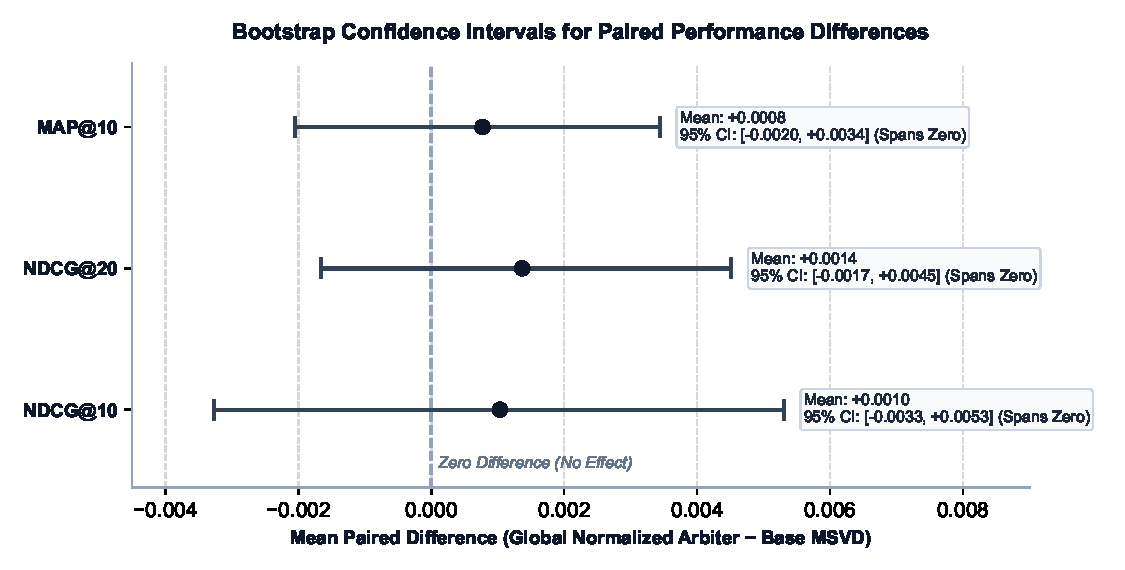
\includegraphics[width=\columnwidth]{bootstrap_confidence_intervals.pdf}
\caption{Bootstrap confidence intervals for paired performance differences ($\text{Global Normalized Arbiter} - \text{Base MSVD}$) across $10{,}000$ resamples. The $95\%$ confidence intervals for NDCG@10 ($[-0.0033, +0.0053]$), NDCG@20 ($[-0.0017, +0.0045]$), and MAP@10 ($[-0.0020, +0.0034]$) all cross zero, confirming that the observed aggregate ranking differences are not statistically distinguishable from zero at the $95\%$ confidence level.}
\label{fig:bootstrap_ci}
\end{figure}

\subsection{Determinism and Multi-Seed Robustness}
We conduct three consecutive independent runs with fixed random seed $42$. The maximum absolute floating-point difference across all ranking metrics is $0.000000$, confirming deterministic metric outputs across the three repeated runs.

Across five initialization seeds ($42, 123, 456, 789, 2026$), the summary statistics are:
\begin{itemize}
    \item \textbf{Base MSVD NDCG@10:} $0.006454 \pm 0.000487$ ($\text{CV} = 7.54\%$, range $[0.005572, 0.006993]$).
    \item \textbf{Global Arbiter NDCG@10:} $0.007721 \pm 0.001056$ ($\text{CV} = 13.68\%$, range $[0.006075, 0.009178]$).
    \item \textbf{Global Arbiter NDCG@20:} $0.007144 \pm 0.000742$ ($\text{CV} = 10.39\%$).
    \item \textbf{Global Arbiter MAP@10:} $0.003381 \pm 0.000698$ ($\text{CV} = 20.64\%$).
\end{itemize}
Across the five evaluated initialization seeds, the Arbiter maintained a higher mean NDCG@10 than Base MSVD, although the Arbiter exhibited greater seed-to-seed variability.

\section{Diversity and Stream Contribution Analysis}

\subsection{Catalog Coverage and Recommendation Diversity}
We evaluate recommendation diversity across the candidate catalog, as detailed in Table~\ref{tab:diversity}.

\begin{table}[t]
\caption{Diversity, Catalog Coverage, and Distributional Metrics (Top-20 Recommendations)}
\label{tab:diversity}
\centering
\begin{tabular}{lcccc}
\toprule
\textbf{Metric} & \textbf{Popularity} & \textbf{Base MSVD} & \textbf{Tag MSVD} & \textbf{Global Arbiter} \\
\midrule
Unique Tracks & $90$ & $7,165$ & $6,772$ & $6,118$ \\
Catalog Coverage (\%) & $0.006\%$ & $0.480\%$ & $0.453\%$ & $0.410\%$ \\
Unique Artists & $38$ & $1,489$ & $931$ & $550$ \\
Artist Coverage (\%) & $0.022\%$ & $0.848\%$ & $0.530\%$ & $0.313\%$ \\
Entropy (bits) & $5.17$ & $12.60$ & $12.49$ & $12.20$ \\
Avg Pop Rank & $1,089$ & $9,614$ & $13,274$ & $21,542$ \\
Pairwise Jaccard & $0.6030$ & $0.0008$ & $0.0011$ & $0.0021$ \\
\bottomrule
\end{tabular}
\end{table}

While Popularity recommends $90$ distinct tracks and $38$ artists with a high pairwise Jaccard similarity of $0.6030$, the Global Normalized Arbiter recommends $6,118$ unique tracks across users with recommendation entropy of $12.20\text{ bits}$ and low inter-user overlap (pairwise Jaccard $= 0.0021$). The Arbiter also yields an average popularity rank of $21,542$ (compared to $9,614$ for Base MSVD).

\subsection{Stream Contribution and Ablations}
To evaluate the contribution of individual streams, we perform ablation by removing individual streams from the normalized arbiter:
\begin{itemize}
    \item \textbf{Full Global Arbiter:} $\text{NDCG@10} = 0.007414$.
    \item \textbf{Ablation without MSVD Stream:} $\text{NDCG@10} = 0.001416$ (Relative drop of $-80.898\%$).
    \item \textbf{Ablation without Tag Stream:} $\text{NDCG@10} = 0.006370$ (Relative drop of $-14.078\%$).
\end{itemize}
This ablation shows that collaborative MSVD serves as the primary ranking component, with the tag stream contributing complementary predictive signal.

\section{Runtime and Computational Scalability}
The system is implemented using sparse CSR/CSC representations in SciPy/NumPy, avoiding dense matrix allocation of the $992 \times 1,493,688$ space. Offline model training and exact retrieval benchmarks are reported in Table~\ref{tab:runtime_benchmarks}.

\begin{table}[t]
\caption{Computational Runtime and Query Latency Benchmarks}
\label{tab:runtime_benchmarks}
\centering
\begin{tabular}{lr}
\toprule
\textbf{Stage / Operational Metric} & \textbf{Authoritative Benchmark} \\
\midrule
Implicit MSVD ALS Training (10 Iterations) & $4,081.8\text{ s}$ ($\approx 68.0\text{ min}$) \\
Tag TF-IDF Sparse Matrix Construction & $389.1\text{ s}$ \\
Temporal Decay Matrix Construction & $266.8\text{ s}$ \\
Full Test Catalog ($1.49\text{M}$ items) Evaluation & $40.9\text{ s}$ \\
\midrule
Single-User Query Latency ($K=5$) & $96.41\text{ ms}$ ($10.37\text{ qps}$) \\
Single-User Query Latency ($K=10$) & $96.48\text{ ms}$ ($10.36\text{ qps}$) \\
Single-User Query Latency ($K=20$) & $96.87\text{ ms}$ ($10.32\text{ qps}$) \\
Batch Latency (50 Users, $K=10$) & $4,824.11\text{ ms}$ \\
Memory Safety Verification & \textbf{Verified Sparse (0 MB Dense)} \\
\bottomrule
\end{tabular}
\end{table}

Single-user top-10 retrieval across the $1.49\text{M}$-item candidate catalog executes in $96.48\text{ ms}$ per query on a single CPU core, delivering $10.36\text{ queries/sec}$ throughput. Top-$K$ selection is performed via partial sorting (\texttt{np.argpartition}) without requiring approximate nearest neighbor index construction.

\section{Explainability Framework}
Because each candidate score $\hat{r}_{ui}$ is a linear combination of normalized components, the system can attribute the final score to collaborative, semantic, and temporal components:
\begin{equation}
\text{Contrib}_{\text{stream}}(u, i) = \frac{w_{\text{stream}} \tilde{s}_{ui}^{\text{stream}}}{\hat{r}_{ui}} \times 100\%.
\end{equation}
These proportional contributions can be exposed as explanation factors for individual recommendations.

\section{Discussion}
The experimental results point to several observations:
\begin{enumerate}
    \item \textbf{Score Normalization in Multi-Stream Fusion:} The unnormalized fixed fusion baseline achieved an NDCG@10 of $0.005932$, whereas the Global Normalized Arbiter reached $0.007414$. This result is consistent with the hypothesis that unnormalized additive fusion is adversely affected by score-scale mismatch across users, and that per-user normalization enables more effective integration of the three streams in the evaluated setting.
    \item \textbf{Auxiliary Signals in Low-Activity Cohorts:} The $+50.472\%$ relative difference in the low-activity cohort ($0.017421$ vs.\ $0.011578$) suggests that social tags and temporal recency kernels can provide useful auxiliary guidance when collaborative interaction histories are sparse.
    \item \textbf{Evaluation at Extreme Catalog Scale:} Evaluating across the unpruned $1.49\text{M}$ candidate catalog reflects realistic ranking conditions. The observed metric magnitudes are consistent with full-catalog ranking without candidate pre-filtering~\cite{cremonesi2010performance}.
\end{enumerate}

\section{Limitations}
We note the following limitations of this study:
\begin{enumerate}
    \item \textbf{Catalog Sparsity and Absolute Metric Scale:} In a $1.49\text{M}$-item catalog with $518$ test users, ground-truth hits per user are sparse, yielding low absolute metric values across all evaluated models.
    \item \textbf{Tag Vocabulary Coverage:} HetRec tags cover $39.7824\%$ of candidate tracks ($594,225$ items). Tracks by unannotated artists receive zero semantic score mass.
    \item \textbf{Artist-Level Semantic Granularity:} Tags are assigned at the artist level, meaning track-specific stylistic variations are not distinguished.
    \item \textbf{Absence of Audio/Acoustic Modeling:} The system does not utilize waveform, acoustic, or deep audio features.
    \item \textbf{Offline Observational Evaluation:} Evaluation is based on observational logs without live online A/B testing or user feedback loops.
    \item \textbf{Scope of Cold Start:} The system does not solve zero-data unseen-item cold start where items have no artist tags or historical interactions.
\end{enumerate}

\section{Future Work}
Future work will explore:
\begin{itemize}
    \item Integrating track-level audio representations derived from self-supervised music audio models.
    \item Investigating non-linear gating functions parameterized by user profile features.
    \item Incorporating session-based models for short-term listening transitions.
\end{itemize}

\section{Conclusion}
This paper presented an evaluation of a Global Normalized Multi-Stream Arbiter recommendation system on the Last.fm 1K dataset across $1,493,688$ candidate tracks. By applying per-user min-max normalization to the collaborative stream, the architecture combines implicit MSVD collaborative factorizations, artist-level HetRec tag TF-IDF profiles, and temporal recency decay signals. Under a strict zero-leakage chronological protocol, the Global Normalized Arbiter achieved an NDCG@10 of $0.007414$, establishing a $+16.384\%$ descriptive gain over Base MSVD, a $+244.648\%$ relative improvement over Popularity ($p = 0.0447, d = 0.1084$), and a $+50.472\%$ descriptive gain for low-activity users, while supporting exact top-$K$ retrieval in $96.48\text{ ms}$ per query with verified sparse memory safety.

\balance
\bibliographystyle{IEEEtran}
\bibliography{references}

\end{document}
